
%=====================================================================
% Document Style
%=====================================================================
% APS format: There is no prescribed format by IIT Bombay
\documentclass{raitspecial}
% To include optional packages, use the \usepackage command.
% For e.g.:
\usepackage{graphicx}
%=======================================================================
% End of Preamble, start of document
%

\begin{document}
% Choose your bibliography style
% plain is the basic style, others include ieeetr, siam, asm, etc
\bibliographystyle{plain}

%\include{defs}                   % Common definitions used throughout the thesis
%============================================================================
% prelude.tex
%   - titlepage
%   - table of contents, list of tables and list of figures
%   - abstract
%============================================================================

\clearpage%
\pagenumbering{roman}  % This makes the page numbers Roman (i, ii, etc)
%--------------------------------------------------------------------%
% TITLE PAGE
%   - define \title{} \author{} \date{}

\title{Study on Fruit Quality Inspection Based on Color Image Processing}
\author{Chitra Sures}

\date{October 2011}

\department{Department of Electronics Engineering}

%    - Set the guide's name
\setguide{Prof. M. D. Patil}
%    - Set the coguide's name (if you have one)
%%\setcoguide{Prof Amitabha Sanyal}

%   - once the above are defined, use \maketitle to generate the titlepage
\maketitle

%--------------------------------------------------------------------
\cleardoublepage \nonumber
\begin{center}

\includegraphics{raitlogo.eps}\\
Ramrao Adik Education Society's\\
\large {\textbf{Ramrao Adik Institute of Technology}}\\
\small(Affiliated to the University of Mumbai)\\
Dr. D. Y. Patil Vidyanagar,Sector 7, Nerul, Navi Mumbai 400
706.\\\vspace{0.3in} \Large CERTIFICATE
\end{center}
\vspace{0.1in}
\begin{center}
\large This to certify that Special Topic Seminar entitled\\
\textbf{\lq\lq Study on Fruit Quality Inspection Based on Color Image Processing\rq\rq} \\submitted by
\begin{center}
Hemlata Kadam (10EL2007)  \\
\end{center}
is approved for the degree of \\ \textbf {Master of Engineering}\\ in\\ \textbf {Electronics Engineering}.\\

 %\vspace{0.5in}
%-----------------------------------------------------------------
%\begin{tabular}{ccc}
%      \rule{6cm}{1sp}                &\rule{10mm}{0pt}& \rule{6cm}{1sp}
%      \\
%       Guide             &&Head of Department \\\\\
%      \rule{6cm}{1sp}                && \rule{6cm}{1sp} \\
%      Examiner 1                 && Examiner 2 \\\\\\
%      Principal: \rule{4cm}{1sp} && \\ && \\
%       &&
%    \end{tabular}
\vspace{1in}
\begin{tabular}{ccc}
      \rule{5cm}{1sp}                &\rule{10mm}{0pt}& \rule{5cm}{1sp}
      \\\vspace{0.5in}
      Examiner 1                 && Examiner 2 \\
      \rule{5cm}{1sp}                && \rule{5cm}{1sp} \\ \vspace{0.5in}
       Guide             && Project Coordinator \\
      \rule{5cm}{1sp}                && \rule{5cm}{1sp} \\
      Head of Department                && Principal \\\\
        %&\rule{5cm}{1sp}& \\
%       &Principal&
    \end{tabular}
\end{center}
%-----------------------------------------------------------------
\cleardoublepage
%--------------------------------------------------------------------%


% ABSTRACT
\begin{abstract}
%\input {abstract}
In this paper, a new method of inspecting fruit
quality is proposed based on color image processing. After an
image of fruits is taken, white balance is performed.Then the
image is transferred from the RGB color model to the HSI
color model. Its simplified histograms of hue H and saturation
S are calculated as the input of a designed BP network. The
output of the BP network is the quality description of the
inspected fruits.After training, the quality of fruits is inspected by the
BP network according to the simplified histograms of H and S
of their color image. Experiments are conducted with the
quality inspection of bananas. Experiment results show the
feasibility and reliability of proposed method.
\end{abstract}

%--------------------------------------------------------------------%
% CONTENTS, TABLES, FIGURES
\tableofcontents \listoftables \listoffigures

%--------------------------------------------------------------------%
%  Single counter for theorems and theorem-like environments:
\newtheorem{theorem}{Theorem}[chapter]
\newtheorem{assertion}[theorem]{Assertion}
\newtheorem{claim}[theorem]{Claim}
\newtheorem{conjecture}[theorem]{Conjecture}
\newtheorem{corollary}[theorem]{Corollary}
\newtheorem{definition}[theorem]{Definition}
\newtheorem{example}[theorem]{Example}
\newtheorem{figger}[theorem]{Figure}
\newtheorem{lemma}[theorem]{Lemma}
\newtheorem{prop}[theorem]{Proposition}
\newtheorem{remark}[theorem]{Remark}

%--------------------------------------------------------------------%
% Make the page numbers Arabic (1, 2, etc)
\cleardoublepage%
\pagenumbering{arabic}
             
\chapter{\textbf{Introduction}}
Stereo vision is an imaging technique that can provide full field of view 3D measurements in an unstructured and dynamic environment. The basic of stereo vision are similar to 3D perception in a human vision and is based on triangulation of rays from multiple viewpoints.\cite{Ed} Each pixel in a digital camera collects the light that reaches the camera along a 3D ray. If feature in the world can be identified as a pixel location in an image then this feature lies on the 3D ray associated with that pixel. If multiple cameras are used multiple rays are obtained. The intersection of these rays is the 3D location of the feature.\\
The key problem to solve stereo vision are to identify which pixel in multiple images match the same world feature .This problem is known as stereo matching or stereo correspondence. Stereo Matching is for a given two or more images of the same scene or object, compute a representation of its shape. Stereo Matching is process of finding disparity or depth information.\cite{Mathias}\\
The tracing of corresponding phenomena i.e. stereo matching is necessary key funtionality in many applications like image sequence analysis in entertainment, information transfer and automated systems. Stereo matching is highly important in fields such as robotics to extract information about the relative position of 3D objects in the vicinity of autonomous systems. Other applications for robotics include object recognition, where depth information allows for the system to separate occluding image components, such as one chair in front of another, which the robot may not be able to distinguish as a separate object by any other criteria.\\
Scientific applications for digital stereo vision include the extraction of information from aerial surveys, for calculation of contour maps or even geometry extraction for 3D building mapping, or calculation of 3D heliographic information such as obtained by the remote sensing projects of the ISRO .

There are many algorithms for stereo matching have been proposed, the computation of disparity still remains challenging in texture less regions, depth discontinuities and occluded areas. The stereo algorithms can be roughly categorized into three classes.\cite{Mu}

The first class is the area-based algorithms. These algorithms attempt to correlate the gray levels of pixels within a finite neighboring window. A central problem of the area- based algorithms is to find the optimal size of the window. While the window size must be large enough to include enough intensity variation for matching, it must be small enough to avoid the effects of projective distortion.
The second class is the feature- based algorithms. They extract features of interest from the image, such as edges, and match the features. The disadvantage of the feature-based algorithms is that they usually yield sparse disparity maps.
The third class global algorithms such as dynamic programming, graph cuts and belief propagation use global constrains over the entire image. Global algorithms can deal with the texture fewer regions and occluded regions well they performed over the whole images.\\
In spite of having advantages of global algorithm, there have been few real time stereo matching implementations due to their high complexity. Among global algorithm, dynamic programming can be used to implement real time systems but is not robust since it doesn't consider vertical consistency\cite{Pearl}
The stereo matching problems can formulate in terms of Markov Random Field as minimum energy function, to find energy minimization function is NP-hard. This means a general solution to this problem will take an unthinkably long time to reach a solution.\\
Belief propagation algorithm is an approach which find the approximate solution for minimum energy functions used for stereo matching.\cite{Chia}
Belief propagation algorithm considers both vertical and horizontal consistency is most robust method in the presence of texture less regions and occlusion .\\
However,Even  Belief propagation is computationally complex and often it implementation in real time is not possible.
Current research is directed towards optimizing the BP algorithms and associated hardware for fast implementation.\cite{aps}


\textbf{Some of the major contributions in the optimization of BP streo matching are as follows:}\\
Chia-Kai et.al\cite{Chia} used Loopy Belief Propagation(LBP)with simple message update process to iteratively refine the beliefs of labels and showed that it could be effectively applied to the  problems like stereo matching, Image de-noising etc..

Pedro F.Felzenszwalb and Daniel P.Huttenlocher \cite{Felzen} used to find cost function by using distance transform technique ,grid graph and perform BP in a coarse to fine method  for solving early vision problem \\
Li Zhou et.al\cite{Li Zhoue} surveyed about  optimization potential for both stereo matching algorithm optimization and software or hardware implementation in terms of speed, parallelism, data bandwidth, memory storage, etc.
The Graphic Processing Unit (GPU), Field Programmable Gate Array (FPGA) and Application-Specific Integrated Circuits (ASIC) designs are future research trends in real time embedded stereo vision application systems because of their high parallel processing capabilities and specific powerful calculation supporting components.\\
Young-kyu Choi et.al\cite{Young} used reducing number of pixels (i.e. reduction in spatial domain) approach is used to reduce data size and transfer bandwidth is significantly reduced by storing only a part of the whole message to optimize the BP.
In order to maintain the accuracy, the local messages are reconstructed by taking advantage of the shared memory available in Graphic Processing Units (GPU)\\
Chi-Hua Lai et.al\cite{Chi-Hua Lai} used  parallelization of a belief propagation algorithm on the multicore processors have proposed. The methods used to demonstrate the issues in optimizing the algorithm by exploiting the potential parallelism to expose the architecture benefits. The methodology of analyzing and exploiting parallelism presented in this article is applicable to other stereo vision algorithms.\\
Eduardo.M et.al\cite{Ed} developed belief algorithm using functional VHDL hardware description language and is technology-independent. So, the system can be implemented on any large enough FPGA \\
Yu-Cheng Tseng et.al\cite{Y.C.} used to partitions an image to block and optimizes with belief propagation which reduces the memory size. The block based approach discontinuous disparities region occurs in the boundary of edges which can enhance the interaction between neighboring blocks such that the independent block could extract useful information from the neighboring finished processing block.\\
Radu Timofte et.al\cite{Radu} used Four-Color Theorem  technique for Belief propagation based on the max-product for solving early vision problems such as MRF problems where energy is to be minimized\\
Nama et.al \cite{Nam Ma} used method task scheduling which is more suitable tool for Parallel implementation of Belief Propagation in Factor Graphs a task dependency graph for belief propagation and then using a dynamic task scheduler to exploit task parallelism available in the task dependency graph.\\
1.2 .Research Problem:  To optimize Belief Propagation algorithm  to reduce computation complexity and increase calculation efficiency.

1.3. Research aim and objective:
To develop Belief Propagation algorithm  to reduce run time and bandwidth for real time applications


1.4.Operatinal definition of terms and concepts.

Some of the Concepts are given  below:

Belief Propagation Techniques approach uses the degree of a person's belief that an event will occur ,rather than the actual probability  of the event will occur.
Belief Propagation Technique is used to perform inference on graphical  model  such as factor graphs which calculates marginal distribution for each unobserved node
conditional on observed node.
Belief Propagation Techniques  are used for performing inference on graphical models such as Bayesian Network and Markov Random Field. In Markov Random  Fields (MRF) the network topology was presumed to be given and problem was to characterize the probabilistic  behavior  of a system complying with dependencies prescribed by network.

Stereo  vision system is three-dimensional (3D) model to give 3D objects using depth information. Stereo matching is concerning on the depth information processing capability. Stereo Matching used to find representation of its shape for a given two or more images of the same scene or object




1.5..Literature Surey:
Some of the major contributions in the optimization of BP stereo matching are as follows:
Chia-Kai et.al[1] used Tile based belief Propagation scheme which reduces memory
 and bandwidth and used another technique fast message construction which reduces the complexity of message construction from quadratic to linear.so it can easily parallelized.
Termination Criteria for Tile based BP are dependent on application and data so it can be possible to apply for some applications like stereo matching

Pedro F.Felzenszwalb and Daniel P.Huttenlocher [2] methods used are first distance transform technique to find new message by using cost function ,other method used are grid graph technique to update the messages.
The third technique used are multi scale algorithm to perform BP in a coarse to fine manner.These techniques are used for solving early vision problems such as stereo ,optical flow and image restoration

Li Zhou et. [3] present a general comparison survey about software and hardware processing algorithms based on algorithm inherent characteristic, implementations, and architectures

optimization potential of an Belief Propagation algorithm measured  in terms of
of speed, parallelism, data bandwidth, memory storage, etc. implemented either for  software or  for hardware
 GPU, FPGA and ASIC designs are  implemented in real-time embedded stereo vision application systems because of their high parallel processing capabilities and specific powerful calculation supporting components.
Implementing GPU has more programming flexible and powerful computational capability than FPGA and ASIC but FPGA and ASIC  have high performance, lower power consumption and cost
Stereo matching system could be enhanced along with software and hardware technology development.


Young-kyu Choi et [4] used novel memory efficient algorithm for BP in which data size and transfer bandwidth is reduced significantly by storing only part of the whole image.
In order to maintain the accuracy, the local messages are reconstructed by Graphic Processing Units (GPU) which is having advantage of available of shared memory.



Chi-Hua Lai e.tc [5] used  method of  parallelization of a belief propagation algorithm on the multicore processors  to optimize the BP  to implement on Graphic Processing Units (GPU).One of the most advanced paradigms is to apply this  technique in inferring the 3-D position of an object for stereo matching .


 Eduardo.M et.all [6] developed a FPGA implementation for depth map estimation using Belief Propagation algorithm for CAFADIS. CAFADIS IS A 3D video camera  patented  by the university of Laguna that performs depth reconstruction in real time.
The main contribution of this work is the use of FPGA technology for processing the huge amount of data



Yu-Cheng Tseng et.a[7]  worked on  a method which is  used  for stereo matching is that by partitioning an image into block and optimize with Belief Propagation. This method reduces the memory storage size with good performance.





Radu  Timofte et.al[8] studied Four-Color Theorem  on Max-product Belief propagation technique. It is used in early computer vision for solving MRF problems where energy is to be minimized

Nama et.al [9]  method used is task parallelism for Belief Propagation in acyclic graphs .The approach for task parallelism consists of constructing a task dependency graph for the input factor graph and then using a task scheduler to allocate tasks to the cores for parallel l execution,






1.6.Research Design:

1. Study the implementation of stereo matching using Belief Propagation and understands the issues in implementation. Study different techniques to optimize belief in different approaches

2. Try to evolve a new approach considering hardware and software implementation in Belief Propagation




1.7.Scope and Limitations:
By using different message passing schemes in belief propagation algorithm can greatly reduces memory, bandwidth and computational time of belief propagation
and enable parallel processing while implementing.

The execution time of belief propagation reduces after certain stability or convergence criteria met ,but termination criteria is application data dependent.

1.8.Tentative Scheme :
The performance of BP algorithm is compared with Mddlebury library is available on line

1.8.Expected Results: Development of a new/modify Belief Propagation optimization method for stereo matching application/cases of stereo matching. Comparative 



\textbf{Problem Definition}:
It is proposed to work on the algorithm optimization and fast implementation of Belief Propagation algorithm without much degradation in accuracy\\

\textbf{Research Design:}
\begin{enumerate}
\item Study the implementation of stereo matching using Belief Propagation and understands the issues in implementation. Study different techniques to optimize belief in different approaches

\item Try to evolve a new approach considering hardware and software implementation in Belief Propagation
\end{enumerate}

\textbf{Expected Results:}

Development of a new/modify Belief Propagation optimization method for stereo matching application/cases of stereo matching. Comparative study of the new method with existing methods.


















            % Chapter 1: Introduction
\chapter{Literature Survey}
%
The major contribution in the field of stereo matching using Random Markov field and inference algorithm like Belief Propagation\newline
\textbf{[2003] Comparison of Graph cuts with Belief Propagation for stereo, Using Identical MRF Parameters:}\cite{r1}\newline
The  disparity image can be achieved  by modelling Markov Random Field and by using optimization algorithm such as Graph cut and Belief Propagation. These two algorithm allow fast and approximate solution to MRF which are powerful tools for modelling vision problems.so one system improvement over the other be attributed to its choice of an inference algorithm.\newline
The comparison between Graph cut algorithm with max product Belief Propagation algorithm shows that the solution for energy  by Graph cut and Belief Propagation  algorithm nearly equal although graph cut consistently returns smaller energy. The solutions produced by Graph cut  are smoother while accelerated Belief Propagation algorithm was faster.\newline
Given this situation Improving formulation of MRF rather than improving solution (optimization algorithm) for MRF.
The comparisons between inference algorithm such as Graph cut and Belief Propagation depends on the functions of MRF formulation.\newline
The future research can be different functions such as truncated linear or quadratic  used for MRF optimizing with any one of the inference algorithm\cite{r1}\newline
\textbf{[2004] Efficient Belief Propagation for Early Vision:}\cite{r2}

The early vision problems such as stereo, optical flow and image restoration can be solved by MRF model by using inference algorithm based on Graph cut and Belief propagation In this paper new algorithm techniques improve the running time of the algorithm.
The inference algorithm used is max product belief propagation.\newline
The three techniques  substantially reduces time required to compute the message updates.
\begin{enumerate}
  \item In low level vision problems the label or hidden node is generally based on some difference between two labels rather than on particular pair of labels, this is known as distance transform technique. This technique reduces message computing time.
  \item In new message update scheme, here nodes are split into two
Messages are updated alternately ,so half of the messages only updated at each iteration.so memory required to store messages are reduced.
\item The third technique uses hierarchical structure to reduce the number of message passing iterations to small constant rather depends on size of the image grid.
\end{enumerate}
\textbf{[2007]   Low Memory Cost Block Based Belief Propagation for Stereo Correspondence}\cite{r3}\newline
The global approaches can handle the texture less and occluded regions well by formulating disparity inference as an energy minimization problem. The energy functions usually has smoothness constraint which represents a certain relationship between neighboring  pixel pair. This smoothness constraint enforces penalty on the energy function, if the labels (disparity or segments)of neighboring pixel are inconsistent.\newline
 The 2D optimization algorithm such as graph cut and Belief Propagation have been applies successfully to optimize energy functions. The BP algorithms construct 2-D graph structures with nodes represent all pixels in the disparity image to find the disparity map with energy closer to the global minima. However, the vast number of nodes in 2-D graph result in extremely high computation complexity too difficulty in real time applications.\newline
The proposed Block based Belief Propagation algorithm directly partitions image into separated independent blocks.so memory size reduces significantly due to block based computation. With block based design, the criterion of convergence becomes important for each block. \newline
In general, the criterion of convergence in belief propagation is defined with the saturation of energy functions. The specific threshold is set to terminate the belief propagation process. However it is difficult to find a global threshold for each block. In proposed algorithm find the convergence according to the equivalence of all disparities for each node in a block over successive iterations.\newline
\textbf{[2009]  Hardware-Efficient Belief Propagation}\cite{r4}\newline
Loopy belief propagation is an effective solution for assigning labels to the nodes of a graphical model such as Markov Random Field, but requires high memory, bandwidth and computational costs.
In this paper two techniques are proposed
\begin{enumerate}
  \item Tile based Belief propagation ,when message is updated data of nodes which are far away are not required, so MRF is divided into
multiple regions known as tile and iterations are done on those regions. So memory required to store messages are reduced.
\item Fast message construction:The cost functions serve for measuring the compatibility between the labels and the observations or prior knowledge.
For example in stereo matching that the disparity values vary smoothly between neighboring pixels. However this assumption is valid only when corresponding pixels belong to the same object. otherwise the difference between their disparity values can be arbitrarily large resulting high cost value. In fast message construction using robust function is used as smmothness cost.

\end{enumerate}
















%
%
%
%%Traditiovnally, diggfital signal processing (DSP) algorithms are
%%implemented using general-purpose (programmable) D
%%in section \ref{organization},we haveeee further,subsection\ref{partt1}
%%\begin{tabular}{|c|c|}
%%                                                                         \hline
%%                                                                         % after \\: \hline or \cline{col1-col2} \cline{col3-col4} ...
%%                                                                         x & y \\
%%                                                                         1 & 2 \\
%%                                                                         \hline
%%                                                                       \end{tabular}







%%%%%%%%%%%%%%%%%%%%%%%%%%%%%%%%%%%%%%%%%%%%%%%%%%%%%%%%%%%%%%%
%\section{Comparison with IR communication}



%%%%%%%%%%%%%%%%%%%%%%%%%%%%%%%%%%%%%%%%%%%table
\begin{table}[h]
\caption{Optimization methods used for finding the disparity from various research papers}
\centering
The summary of literature survey is mentioned in table
\begin{tabular}{|p{1in}|p{2in}|p{2in}|}
%%\begin{tabular}{|c|c|c|}

%\caption{Comparison of short-range wireless communication technologies (FIR fast infrared, VFIR very fast infrared).}
  \hline
  % after \\: \hline or \cline{col1-col2} \cline{col3-col4} ...
  Research paper & Optimization Method & Scope for Research \\
  \hline
  Comparison of Graph cuts with Belief Propagation for stereo, Using Identical MRF Parameters
[2003]
 & Comparative study of Graph cut and Belief Propagation on same MRF Model& Further study of
Improving formulation of MRF rather than improving solution for MRF
 \\
  \hline
  Efficient Belief Propagation for Early Vision
[2004]
 &Three methods are used\begin{enumerate}
     \item Distance transform technique(difference between two labels)
     \item New message update scheme
     \item Hierarchical structure
   \end{enumerate}
  & Further study can be:
These optimization method can be
applicable to a broad range of more sophisticated cost functions.
 \\
  \hline
  Low Memory Cost Block Based Belief Propagation for Stereo Correspondence
[2007]
 & 2D BP Graph is divided into blocks. Optimize each block separately. & The information exchange between Neighboring finished processing block and unfinished processing block can be  further investigated \\
 \hline
 Hardware-Efficient Belief Propagation
[2009]
 & Efficiency of BP is improved by new message scheme known as Tile based BP and Fast message construction & The performance Tile based message passing scheme can be studied for different conditions  like different smoothness cost functions \\
%  \hline
%  Security & Good & Good \\
%  \hline
%  Carrier wavelength (frequency) & 380$~$780 nm visible light (multiple wavelengths) & 850 nm infrared \\
%  \hline
%  Services & Communication, illumination & Communication \\
%  \hline
%  Noise Source & Sun light, Other illumination & Ambient light \\
%  \hline
%  Environmental & Daily usage Eye safe (visible) & Eye safe for low power (invisible) \\
%  \hline
%  Applications & Indoor vehicular communication, Optical ID & Remote control, Point to point connection \\
  \hline
\end{tabular}
\label{table:comp}
\end{table}
                   % Other chapters as required

\chapter{Mathematical Representation of Global stereo Algorithm}

The stereo matching problem can be expressed as global function .The optimization technique used by this global function are by combining matching cost and smoothness cost terms and possibly other terms to get disparity map.
Stereo matching problem can be interpreted in terms of probability theory as well as markov network.
\section{Stereo matching in terms of Probability theory}
The stereo matching problem can be expressed  in terms of probability theory\begin{itemize}
\item Let assume Y is stereo set and X is disparity map
\item Probability of disparity map to stereo set is $P(X/Y)$,Probability of disparity map is $P(X)$ and
Probability of stereo set is $P(Y)$

\item According to Bays theorem from probability theory is
\begin{equation}\label{}
    P(X/Y) = P(Y/X)*P(X)/P(Y)
\end{equation}
\item  Probability of stereo set i.e.$P(Y)$ can made equal to 1
\item Than
\begin{equation}\label{}
    P(X/Y) = P(Y/X)*P(X)
\end{equation}

\end{itemize}
The disparity map can be obtained by maximizing probability of disparity map to stereo set i.e.$P(X/Y)$ and it can be possible by expressing probability into function.
\subsection{Matching cost function}
The probability of stereo set to disparity map i.e.$P(Y/X)$ represents total matching cost across all pixels in stereo set. When probability of stereo set to disparity map i.e.$P(Y/X)$ is low than total matching cost is more and viceversa. \newline Therefore probability of stereo set to disparity map i.e.$P(Y/X)$ can be expressed as function
\newline Abbrevations used in equations are Matching cost=M.C,Smoothing Cost =S.C,Disparity Map=D.M.
\begin{equation}\label{}
Datacost=\prod \limits_{All\enspace pixels\enspace\textbf{s}in D.M}e^{-1*\{M.C\enspace of \enspace\textbf{s}\enspace given\,\textbf{d\_s} \enspace in \enspace D.M\}}
\end{equation}
The value of probability of stereo set to disparity map .i.e.(Y/X) is between 0 to 1.
\begin{enumerate}

  \item If matching cost of all pixels is 0, than probability of stereo set to disparity map.i.e.(Y/X) is 1 since $\exp^0$ is 1

  \item If matching cost of any pixel is 1, than probability of stereo set to disparity map.i.e. (Y/X) is 0  since $\exp^\infty$  is 0

\end{enumerate}
Therefore as matching cost of pixels increase, probability of stereo set to disparity map .i.e. (Y/X) decreases.
\subsection{Smoothness cost function}
The probability of disparity map i.e. P(X) represents total smoothness cost of disparity map. When pixels near each other have the same disparity, smoothness cost\enspace i.e. P(X) is 1 and vice versa. Therefore smoothness cost and probability of disparity map are inversely related.
The probability of disparity map i.e. (X) can be expressed as a function
\begin{equation}\label{}
Datacost=\prod \limits_{All 4 connected\enspace neighbouring pixels \textbf{s,t,}in \enspace D.M.}e^{-1*\{S.C. between sandt given \textbf{d\_s \& d\_t} }
\end{equation}
The probability of disparity map i.e. P(X) does not depends on stereo set. The disparity of all pixels in disparity map is constant regardless of any stereo set
The probability of stereo set to disparity map .i.e. P(Y/X) and the probability of disparity map i.e. P(X) is expressed as matching cost term and smoothness cost term.
The global stereo methods finds disparity map as a minimizing energy function for disparity values. The global stereo methods formulated as an energy minimization which uses data term and smoothes term as objective function.
\subsection{Models for matching and smoothness cost}
The data cost   is based on the intensity differences between the two pixels. The Sum of Absolute Difference (ABS) or Sum of Square Difference (SSD) functions are used as data cost.
The smoothness cost or sometimes referred to as the pairwise term which compares adjacent pixels. Most commonly used smoothness cost functions used as smoothness cost models are Pott's model, linear and quadratic models
The Pott's model is a binary penalizing function with a single tunable    variable. This value controls how much smoothing is applied. The linear and quadratic models have an extra parameter K. K is a truncation value that caps the maximum penalty.
\begin{figure}[h]
\begin{center}
\includegraphics[width=3.5in]{SM.eps}
\caption{Pott's model, Linear and Quadratic models} \label{lined}
\end{center}
\end{figure}
\section{Markov network}
The stereo matching problem can be expressed as markov network. The markov network model is a probability graphical model which consists of undirected graph of 'n' nodes with pair wise potentials as compatibility function.

\begin{itemize}
  \item The state of each nodes  $'i'$ represent as \textbf{X}\_i for given evidence \textbf{Y} Now, Joint compatibility function for markov network is $\Phi(\textbf{X}\_s, \textbf{Y})$
  \item Whereas $X\_s$ is hidden node state, Y is evidence or observed state node,Compatibility function for markov network is $\Psi$(\textbf{X}\_s, \textbf{X}\_t)
  \item If node pair is not compatible, than compatibility between neighboring nodes $X\_s$, $X\_t$ is small.
  \item To find most likely set of nodes $\{X\_1, X\_2, X\_n\}$ for given evidence 'Y' and compatibility between neighboring nodes can be expressed as a joint probability distribution function of $n$ nodes.
\end{itemize}
\begin{equation}\label{}
    P (X\_1, X\_2, X\_n/Y) =\prod \limits_{All nodes \textbf{s}}\Phi(X\_s ,Y ) \prod\limits_{(All neighboring of nodes \textbf{s,t})}\Phi(X\_s ,X\_t )
\end{equation}
Now the goal is to find set of nodes that maximizes joint probability distribution.
\begin{figure}[h]
\begin{center}
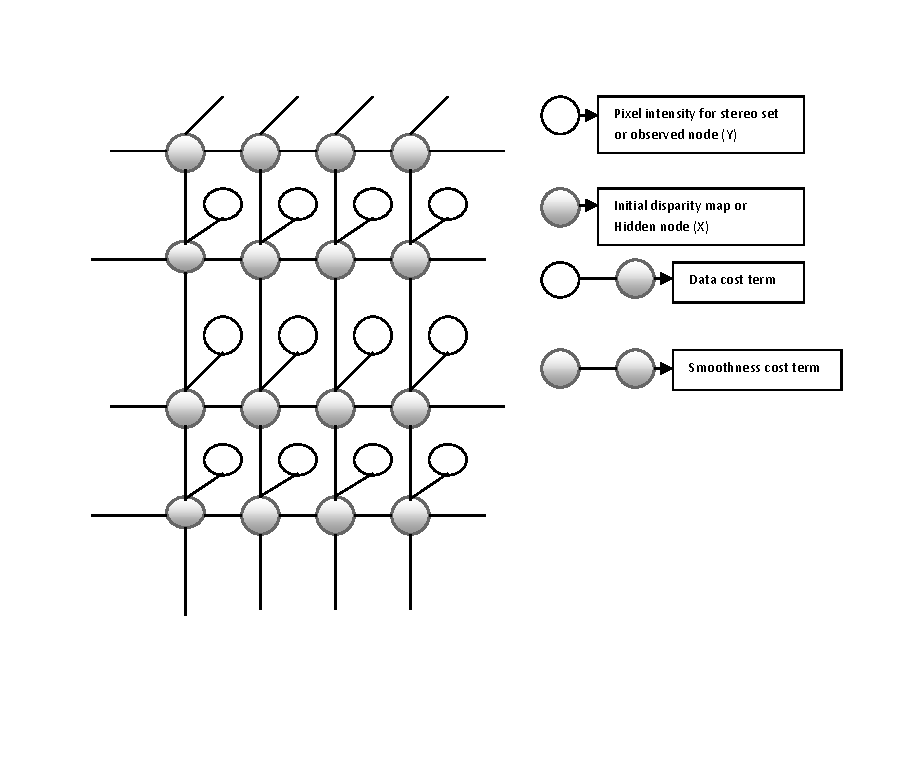
\includegraphics[width=5.5in]{markov.eps}
\caption{Stereo matching problem in Markov Representation } \label{lined}
\end{center}
\end{figure}

\begin{table}[h]
\caption{Stereo matching problem as probability theory and markov network }
\centering
Comparison of probability theory and Markov network are mentioned in table
\begin{tabular}{|p{1in}|p{2in}||p{3in}|}
\hline
  % after \\: \hline or \cline{col1-col3} \cline{col4-col5} ...
S.No.&Probability Theory & Markov network \\
  \hline
1& Maximizing probability of disparity map to stereo set i.e. $P(X/Y)$
 & Maximizing joint probability distribution i.e.
$P(X_1 ,X_2,�..X_n/Y)$ \\
\hline
 2& Set of pixels in disparity map each with assigned  disparity value
& Markov state \\
\hline
3&For given set of stereo images & For given Evidence Y \\
\hline
\end{tabular}
\label{table:comp}
\end{table}
Now stereo problem is reduce to finding Maximum A Posteriori (MAP) estimation in markov network.\newline To find Maximum A Posteriori (MAP) estimation in markov network is NP hard means to get a solution for such problem takes unthinkably long time which is because each pixel (node) in disparity map can take any value in disparity space (state).
\newline  Graph cuts and Belief Propagation are two global methods used to estimate Maximum a Posteriori (MAP) in reasonable amount of time
\section{Belief propagation}
The belief propagation algorithm was proposed by Pearl in 1988 for finding exact marginal's on graphs known as trees that contain no loops. The same concepts can be applied to the graphs which contains loops known as Loopy belief propagation.\newline The Loopy belief propagation is an approximate inference algorithm which keep passing the messages around markov state or node until stable belief state is reached, so the Loopy belief propagation algorithm is an iterative algorithm, messages will converge on doing iterations.\newline
There are three main steps finding Maximum a Posteriori (MAP) estimation or beliefs in markov network.
\begin{enumerate}
  \item 	Normalization
  \item 	Message update or generation
  \item  	Finding belief
\end{enumerate}
\begin{enumerate}
  \item \textbf{Normalization} is required because while continuously multiplying probabilities, messages becomes zero and hits the floating point limits. The normalization is difference of stereo set (observed node in markov network) to Initial disparity (hidden node in markov network) and divided by 256 for 8 bit brightness or gray level representation.
  \item \textbf{In Message updates or generation }step messages are updated by joint probability of data cost, smoothness cost and for all incoming messages which are marginalized over given disparity. Initially messages are updated or generated for right movement and similarly for up, left and for down movements. All these four movements of messages in message update step are in sum product approach. The Loopy belief propagation also known as Sum product algorithm.\newline
The final message in message update or generation step is a vector and size of the vector depends on disparity value.

  \item \textbf{In finding belief step,} the values of belief can be found either by Max Product belief propagation     or by Minimum of Sum belief propagation.
\end{enumerate}
\begin{figure}[h]
\begin{center}
\includegraphics[width=3.5in]{bp1.eps}
\caption{Flow chart for Belief Propagation } \label{lined}
\end{center}
\end{figure}



The best assignment of disparity can be assigned in maximum a posteriori (MAP) by finding largest marginal probability. The belief value in maximum a posteriori (MAP) at each node or state is maximum marginal.\newline
One of the important assumptions of Max Product belief propagation algorithm is belief values or maximum marginal values at each node or state are different. The belief values are converging by iterating Max Product belief propagation algorithm. The optimal assignment for maximum a posteriori (MAP) is depends on the number of iterations.




%\begin{tabular}{|Research paper|Optimization Method|Scope for Research|}
%  \hline
%  % after \\: \hline or \cline{col1-col2} \cline{col3-col4} ...
%   &  &  \\
%   &  &  \\
%   &  &  \\
%   &  &  \\
%  \hline
%\end{tabular}
%%

                   % Other chapters as required
\chapter{Introduction}
\label{ChapterIntroduction}
%\renewcommand{\baselinestretch}{1.5}\normalsize
%
dbfvdjkhskjb lguuklrjkljknnn,mvn,n,nvkndknvkh

%\begin{figure}[h]
%\begin{center}
%\includegraphics[width=4.0in]{drawing-1.eps}
%\caption{m2m.} \label{scenory}
%\end{center}
%\end{figure}
%%                   % Other chapters as required
%\include{chap_conclusions}      % Finally the summary & conclusions

%--------------------------------------------------------------------%
% APPENDIX
%  Appendices, if any, must precede the cited literatures.
%  Appendices shall be numbered in Roman Capitals (e.g. Appendix IV)
\appendix
%\include{appendix_1}        % Appendices if any..

%--------------------------------------------------------------------%
% LITERATURE CITED
%   This should follow the appendices, if any, otherwise summary and
%   conclusions chapter.
\bibliography{xyz}              % Make the bibliography

%--------------------------------------------------------------------%
% ACKNOWLEDGMENTS
%   For APS, acknowledgements can be the first item after title page
%      OR
%   the very last item.
%
\begin{acknowledgments}
I thank the many people who have done lots of nice things for me.
\end{acknowledgments}


\end{document}
